% ============================================================
%  Thesis Progress Slides
%  Cross-Lingual Anti-Christian Hate Speech: Who, How, Why
%  Zhidian Huang | University of Zurich
% ============================================================
\documentclass[aspectratio=169,10pt]{beamer}

% ── Theme ────────────────────────────────────────────────────
\usetheme{Madrid}
\usecolortheme{default}

% Custom colour palette (UZH blue + warm accent)
\definecolor{uzh}{RGB}{0,40,165}
\definecolor{uzhlight}{RGB}{220,230,255}
\definecolor{accent}{RGB}{220,80,30}
\definecolor{accentlt}{RGB}{255,235,220}
\definecolor{darkgray}{RGB}{60,60,60}
\definecolor{enzh}{RGB}{70,130,180}    % steel blue for EN
\definecolor{zhcol}{RGB}{255,140,0}    % orange for ZH
\definecolor{jacol}{RGB}{60,160,80}    % green for JA

\setbeamercolor{palette primary}{bg=uzh,fg=white}
\setbeamercolor{palette secondary}{bg=uzh!80,fg=white}
\setbeamercolor{palette tertiary}{bg=uzh!60,fg=white}
\setbeamercolor{palette quaternary}{bg=uzh,fg=white}
\setbeamercolor{structure}{fg=uzh}
\setbeamercolor{section in toc}{fg=uzh}
\setbeamercolor{alerted text}{fg=accent}
\setbeamercolor{block title}{bg=uzh,fg=white}
\setbeamercolor{block body}{bg=uzhlight}
\setbeamercolor{block title alerted}{bg=accent,fg=white}
\setbeamercolor{block body alerted}{bg=accentlt}
\setbeamercolor{frametitle}{bg=uzh,fg=white}

% ── Packages ─────────────────────────────────────────────────
\usepackage{graphicx}
\usepackage{booktabs}
\usepackage{colortbl}
\usepackage{multirow}
\usepackage{xcolor}
\usepackage{tikz}
\usetikzlibrary{arrows.meta,positioning,shapes.geometric,fit,backgrounds,calc, patterns}
\usepackage{pgfplots}
\pgfplotsset{compat=1.18}
\usepackage{amsmath,amssymb}
\usepackage{pifont}
\usepackage{array}
\usepackage{tabularx}
\usepackage[numbers,sort&compress]{natbib}

% Simple icon substitutes
\newcommand{\faCheckCircle}{\ding{52}}
\newcommand{\faExclamationTriangle}{$\blacktriangle$}
\newcommand{\highlight}[1]{{\color{accent}\textbf{#1}}}

% ── Graphics path (relative to report/) ──────────────────────
\graphicspath{{\subfix{../images/}}}

% ── Beamer settings ──────────────────────────────────────────
\setbeamerfont{title}{size=\Large,series=\bfseries}
\setbeamerfont{subtitle}{size=\normalsize}
\setbeamerfont{frametitle}{size=\normalsize,series=\bfseries}
\setbeamertemplate{navigation symbols}{}
\setbeamertemplate{footline}[frame number]

% ── Metadata ─────────────────────────────────────────────────
\title{Cross-Lingual Anti-Christian Hate Speech}
\subtitle{Who Attacks, How, and Why --- A Trilingual Computational Analysis}
\author{Zhidian Huang}
\institute{Department of Computational Linguistics \textperiodcentered\ University of Zurich}
\date{\today}

% ── Reusable TikZ styles ─────────────────────────────────────
\tikzset{
  mbox/.style={rectangle,rounded corners=4pt,draw=uzh,fill=uzhlight,
               text width=#1,align=center,minimum height=0.9cm,font=\small},
  mbox/.default=2.8cm,
  sbox/.style={rectangle,rounded corners=3pt,draw=gray!60,fill=white,
               text width=#1,align=center,font=\scriptsize,inner sep=3pt},
  sbox/.default=2.6cm,
  arr/.style={-{Stealth[length=5pt]},very thick,color=uzh},
}

% ============================================================
\begin{document}
% ============================================================

% ── SLIDE 1 · Title ──────────────────────────────────────────
\begin{frame}[plain]
  \titlepage
\end{frame}

% ── SLIDE 2 · Roadmap ────────────────────────────────────────
\begin{frame}{Roadmap}
  \begin{columns}[t]
    \begin{column}{0.5\textwidth}
      \tableofcontents[sections={1-3}, hideallsubsections]
    \end{column}
    \begin{column}{0.5\textwidth}
      \tableofcontents[sections={4-8}, hideallsubsections]
    \end{column}
  \end{columns}
\end{frame}

\section{Background \& Research Questions}
\section{Data \& Augmentation}
\section{Analytical Pipeline \& BERTopic}
\section{RQ1 --- Who? Method \& Results}
\section{RQ2 --- How? Method \& Results}
\section{RQ3 --- Why? Method \& Results}
\section{Discussion}
\section{Contributions, Limitations \& Outlook}

% ============================================================
\section{Background \& Research Questions}
% ============================================================

% ── SLIDE 3 · Motivation ─────────────────────────────────────
\begin{frame}{The Problem in One Sentence}
  \begin{center}
    \large
    \textit{``Hate speech research talks a lot about \highlight{what} people say.\\[6pt]
    We ask \highlight{who} they attack, \highlight{how}, and \highlight{why}.''}
  \end{center}
  \vspace{6pt}
  \begin{columns}[T]
    \column{0.48\textwidth}
      \begin{block}{Three blind spots in the literature}
        \begin{itemize}
          \item \textbf{English-centric} corpora dominate
          \item \textbf{Binary} hate/not-hate is the default task
          \item \textbf{Anti-Christian} discourse in East Asia barely studied
        \end{itemize}
      \end{block}
    \column{0.48\textwidth}
      \begin{alertblock}{This thesis}
        Builds a \textbf{trilingual} (EN / ZH / JA)\\
        interpretable analytical pipeline ---\\[4pt]
        \quad from \emph{detection}\\
        \quad to structured \emph{discourse analysis}
      \end{alertblock}
  \end{columns}
\end{frame}

% ── SLIDE 4 · Research Questions ─────────────────────────────
\begin{frame}{Three Linked Research Questions}
  \begin{center}
  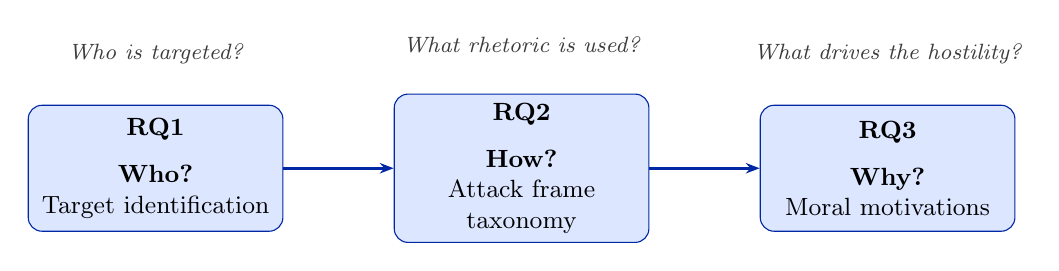
\begin{tikzpicture}[
    rqbox/.style={rectangle,rounded corners=5pt,draw=uzh,fill=uzhlight,
                  text width=3.0cm,align=center,minimum height=1.6cm,font=\small},
  ]
    \node[rqbox] (r1) {\textbf{RQ1}\\[6pt]\textbf{Who?}\\Target identification};
    \node[rqbox,right=1.4cm of r1] (r2) {\textbf{RQ2}\\[6pt]\textbf{How?}\\Attack frame taxonomy};
    \node[rqbox,right=1.4cm of r2] (r3) {\textbf{RQ3}\\[6pt]\textbf{Why?}\\Moral motivations};
    \draw[arr] (r1)--(r2);
    \draw[arr] (r2)--(r3);
    \node[above=0.4cm of r1,font=\footnotesize\itshape,text=darkgray] {Who is targeted?};
    \node[above=0.4cm of r2,font=\footnotesize\itshape,text=darkgray] {What rhetoric is used?};
    \node[above=0.4cm of r3,font=\footnotesize\itshape,text=darkgray] {What drives the hostility?};
  \end{tikzpicture}
  \end{center}
  \vspace{6pt}
  \begin{block}{}
    \centering\small
    Case study: \textbf{anti-Christian discourse} in Chinese, Japanese \& English ---\\
    the \emph{same target} appears across very different cultural contexts.
  \end{block}
\end{frame}

% ============================================================
\section{Data \& Augmentation}
% ============================================================

% ── SLIDE 5 · Corpus ─────────────────────────────────────────
\begin{frame}{A Trilingual Corpus --- Built from Scratch}
  \begin{columns}[T]
    \column{0.40\textwidth}
      \begin{block}{Corpus at a glance}
        \centering\vspace{4pt}
        \begin{tabular}{lrr}
          \toprule
          Lang & Texts & Source \\
          \midrule
          \textbf{EN} & 58,940 & 4 public datasets \\
          \textbf{ZH} & 1,965  & Tieba (crawled) \\
          \textbf{JA} & 2,360  & 5ch (crawled) \\
          \midrule
          \textbf{Total} & \textbf{63,265} & \\
          \bottomrule
        \end{tabular}
        \vspace{4pt}
      \end{block}
      \vspace{4pt}
      \footnotesize
      EN: filtered from HateXplain, Jigsaw,\\
      MLMA, Measuring Hate Speech\\[4pt]
      ZH/JA: manual annotation (Label Studio)\\
      + LLM localization (back-translation)
    \column{0.56\textwidth}
      \begin{alertblock}{The low-resource challenge}
        ZH and JA hate speech data is scarce.\\
        Naively-trained classifiers perform very poorly.
      \end{alertblock}
      \vspace{6pt}
      \begin{block}{Two-stage pipeline for ZH / JA}
        \textbf{Stage 1 --- Native:}
        \begin{itemize}\small
          \item Crawl \textrightarrow\ Manual annotation \textrightarrow\ Fine-tune classifier (Focal Loss)
        \end{itemize}
        \textbf{Stage 2 --- Augmentation:}
        \begin{itemize}\small
          \item Translate EN seed texts into ZH/JA
          \item Filter with the same classifier
        \end{itemize}
      \end{block}
      \vspace{4pt}
      \footnotesize\color{accent}
      \textit{Key failure:} LLM seed-guided generation collapses into\\
      keyword loops after 20--30 iterations\\
      (JA: 100\% redundant at 30 samples; ZH: 90\% at 50)\\
      $\Rightarrow$ back-translation is more robust.
  \end{columns}
\end{frame}

% ── SLIDE 6 · Augmentation results ───────────────────────────
\begin{frame}{Data Augmentation: Three Strategies, One Clear Winner}
  \begin{columns}[T]
    \column{0.55\textwidth}
      \vspace{2pt}
      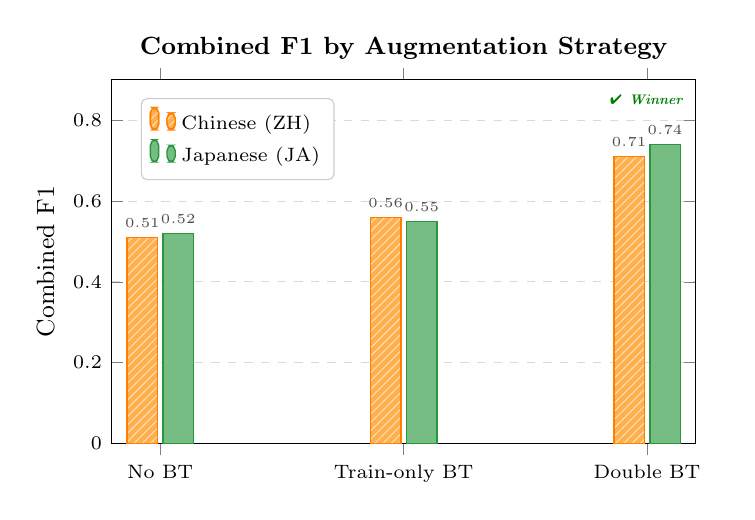
\begin{tikzpicture}
        \begin{axis}[
          ybar, bar width=11pt,
          width=9cm, height=6.2cm,
          ylabel={\small Combined F1},
          ymin=0, ymax=0.90,
          symbolic x coords={
            {No BT},
            {Train-only BT},
            {Double BT}
          },
          xtick=data,
          x tick label style={font=\scriptsize, align=center, text width=1.8cm},
          ytick={0,0.2,0.4,0.6,0.8},
          yticklabel style={font=\scriptsize},
          ymajorgrids=true,
          grid style={dashed, gray!30},
          legend style={
            at={(0.05,0.95)}, anchor=north west,
            font=\scriptsize, cells={anchor=west},
            draw=gray!40, fill=white, rounded corners=2pt,
            inner sep=3pt
          },
          title={\small\bfseries Combined F1 by Augmentation Strategy},
          title style={yshift=-2pt},
          nodes near coords,
          nodes near coords align={vertical},
          every node near coord/.append style={
            font=\tiny\bfseries,
            /pgf/number format/fixed,
            /pgf/number format/precision=2,
            color=black!70,
          },
        ]
          % Chinese bars
          \addplot[
            fill=zhcol!70, draw=zhcol!110, line width=0.5pt,
            postaction={pattern=north east lines, pattern color=zhcol!30}
          ] coordinates {
            ({No BT},      0.51)
            ({Train-only BT}, 0.56)
            ({Double BT},  0.71)
          };
          % Japanese bars
          \addplot[
            fill=jacol!70, draw=jacol!110, line width=0.5pt,
          ] coordinates {
            ({No BT},      0.52)
            ({Train-only BT}, 0.55)
            ({Double BT},  0.74)
          };
          \legend{Chinese (ZH), Japanese (JA)}

          % Annotate Double BT as winner
          \node[
            font=\tiny\bfseries, color=green!50!black,
            above=2pt
          ] at (axis cs:{Double BT}, 0.80) {\faCheckCircle~\textit{Winner}};
        \end{axis}
      \end{tikzpicture}

    \column{0.41\textwidth}
      \vspace{4pt}

      \begin{block}{Strategy A --- No BT}
        \small Raw annotations only.\\[1pt]
        \textit{Data scarcity limits ceiling;\\
        Combined F1\,$\approx$\,0.51.}
      \end{block}

      \begin{block}{Strategy B --- Train-only BT}
        \small Augment training set only.\\[1pt]
        \textit{Synthetic train\,$\neq$\,natural eval\\
        $\Rightarrow$ distribution shift, F1\,$\approx$\,0.56.}
      \end{block}

      \begin{alertblock}{\faCheckCircle~Strategy C --- Double BT}
        \small Back-translate \textbf{both} sets.\\
        Eliminates distribution gap.\\[5pt]
        \highlight{ZH:\;$0.51\;\to\;0.71$\;({\color{green!60!black}$+39\%$})}\\[2pt]
        \highlight{JA:\;$0.52\;\to\;0.74$\;({\color{green!60!black}$+42\%$})}
      \end{alertblock}

  \end{columns}
\end{frame}

% ============================================================
\section{Analytical Pipeline \& BERTopic}
% ============================================================

% ── SLIDE 7 · Pipeline overview ──────────────────────────────
\begin{frame}{The Who--How--Why Pipeline}
  \begin{center}
  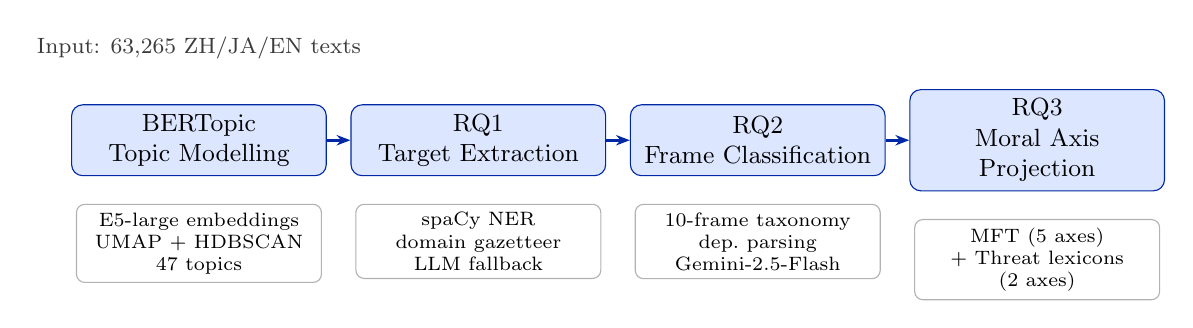
\begin{tikzpicture}[node distance=1.2cm]
    \node[mbox=3.0cm] (bt)  {BERTopic\\Topic Modelling};
    \node[mbox=3.0cm,right=0.3cm of bt]  (r1) {RQ1\\Target Extraction};
    \node[mbox=3.0cm,right=0.3cm of r1]  (r2) {RQ2\\Frame Classification};
    \node[mbox=3.0cm,right=0.3cm of r2]  (r3) {RQ3\\Moral Axis Projection};

    \draw[arr] (bt)--(r1);
    \draw[arr] (r1)--(r2);
    \draw[arr] (r2)--(r3);

    \node[sbox=2.9cm,below=0.35cm of bt]
      {E5-large embeddings\\UMAP + HDBSCAN\\47 topics};
    \node[sbox=2.9cm,below=0.35cm of r1]
      {spaCy NER\\domain gazetteer\\LLM fallback};
    \node[sbox=2.9cm,below=0.35cm of r2]
      {10-frame taxonomy\\dep.\ parsing\\Gemini-2.5-Flash};
    \node[sbox=2.9cm,below=0.35cm of r3]
      {MFT (5 axes)\\+ Threat lexicons\\(2 axes)};

    \node[above=0.45cm of bt,font=\footnotesize,text=darkgray]
      {Input: 63,265 ZH/JA/EN texts};
  \end{tikzpicture}
  \end{center}
  \vspace{4pt}
  \begin{block}{}
    \small\centering
    \textbf{Design principle:} thematic structure is \emph{induced} from the corpus (not imposed),\\
    so findings are not pre-biased toward English-language research assumptions.
  \end{block}
\end{frame}

% ── SLIDE 8 · BERTopic results ────────────────────────────────
\begin{frame}{BERTopic: 47 Cross-Lingual Topics}
  \begin{columns}[T]
    \column{0.60\textwidth}
      \vspace{2pt}
      
\includegraphics[width=\linewidth]{images/foundations/datamap_bertopic_labelled_cluster.png}
      {\tiny Document map. Each point = one text; colours = topic cluster.}
    \column{0.36\textwidth}
      \begin{block}{Key numbers}
        \small
        \begin{tabular}{ll}
          Topics found & \textbf{47} \\
          Noise docs   & 2,530 (4\%) \\
          Largest topic & 499 docs \\
        \end{tabular}
      \end{block}
      \begin{block}{Monolingual topics}
        {\footnotesize
        \begin{itemize}
          \item JP (99\%): Unification Church \& Abe
          \item EN (92\%): Religion \& Canadian identity
          \item ZH (96\%): Missionaries in China
        \end{itemize}}
      \end{block}
      \begin{alertblock}{Cross-lingual (entropy $\approx$1.1)}
        {\footnotesize
        \begin{itemize}
          \item LGBTQ+ \& Catholic teaching
          \item Science vs.\ creationism
          \item Conservative/liberal church split
        \end{itemize}}
      \end{alertblock}
  \end{columns}
\end{frame}

% ============================================================
\section{RQ1 --- Who? Method \& Results}
% ============================================================

% ── SLIDE 9 · RQ1 Method ─────────────────────────────────────
\begin{frame}{RQ1 --- Method: Three-Stage Target Extraction}
  \begin{center}
    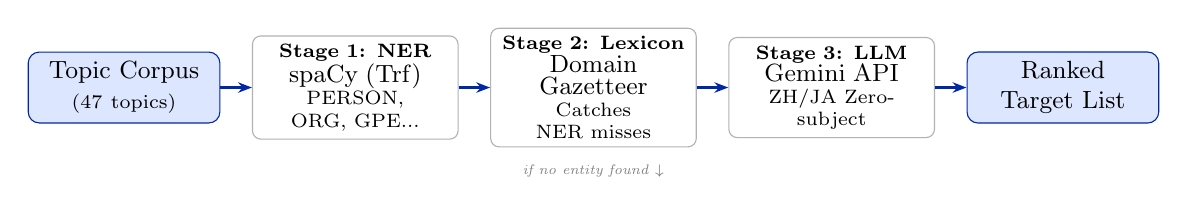
\begin{tikzpicture}[node distance=0.3cm and 0.4cm]
        % 定义节点宽度，让视觉更统一
        \tikzset{
            mbox/.append style={text width=2.2cm},
            sbox/.append style={text width=2.4cm}
        }
    
        \node[mbox] (inp) {Topic Corpus\\{\scriptsize (47 topics)}};
    
        \node[sbox, right=of inp] (s1) {
            \textbf{Stage 1: NER}\\
            {\small spaCy (Trf)}\\
            {\scriptsize PERSON, ORG, GPE...}
        };
    
        \node[sbox, right=of s1] (s2) {
            \textbf{Stage 2: Lexicon}\\
            {\small Domain Gazetteer}\\
            {\scriptsize Catches NER misses}
        };
    
        \node[sbox, right=of s2] (s3) {
            \textbf{Stage 3: LLM}\\
            {\small Gemini API}\\
            {\scriptsize ZH/JA Zero-subject}
        };
    
        \node[mbox, right=of s3] (out) {Ranked\\Target List};
    
        % 连线
        \draw[arr] (inp) -- (s1);
        \draw[arr] (s1) -- (s2);
        \draw[arr] (s2) -- (s3);
        \draw[arr] (s3) -- (out);
    
        % 注释简化
        \node[font=\tiny\itshape, text=gray, below=0.1cm of s2] {if no entity found $\downarrow$};
    \end{tikzpicture}
  \end{center}
  \vspace{6pt}
  \begin{block}{}
    \small\centering
    A \textbf{blacklist} removes pronouns and generic religious nouns (``faith'', ``religion'')\\
    that appear universally and carry no discriminative information about specific targets.
  \end{block}
\end{frame}

% ── SLIDE 10 · RQ1 top targets ───────────────────────────────
\begin{frame}{RQ1 --- Results: Top-20 Targets per Language}
  \begin{center}
    
\includegraphics[width=0.93\textwidth]{images/RQ1/rq1_global_top20_bilingual.png}
  \end{center}
  {\tiny Top-20 hate-speech targets per language, ranked by total mention frequency. Labels: original language + English translation.}
\end{frame}

% ── SLIDE 11 · RQ1 category heatmap ──────────────────────────
\begin{frame}{RQ1 --- Results: Target Profiles Differ by Language}
  \begin{columns}[T]
    \column{0.55\textwidth}
      
\includegraphics[width=\linewidth]{images/RQ1/rq1_lang_category_heatmap.png}
      {\tiny Target-category frequency heatmap by language.}
    \column{0.42\textwidth}
      \vspace{6pt}
      \begin{block}{Language-specific patterns}
        \small
        \textbf{English} --- \emph{clergy} dominate; named individuals prominent\\[4pt]
        \textbf{Chinese} --- \emph{church institutions} \& historical missionaries; state-framed discourse\\[4pt]
        \textbf{Japanese} --- \emph{Unification Church} as focal point; political entanglement salient
      \end{block}
      \vspace{6pt}
      \begin{alertblock}{Key finding}
        \small Attack targets reflect each community's \textbf{socio-political context},\\
        not just shared religious subject matter.
      \end{alertblock}
  \end{columns}
\end{frame}

% ============================================================
\section{RQ2 --- How? Method \& Results}
% ============================================================

% ── SLIDE 12 · RQ2 Method ────────────────────────────────────
\begin{frame}{RQ2 --- Method: Three-Layer Predicate Extraction}
  \begin{center}
    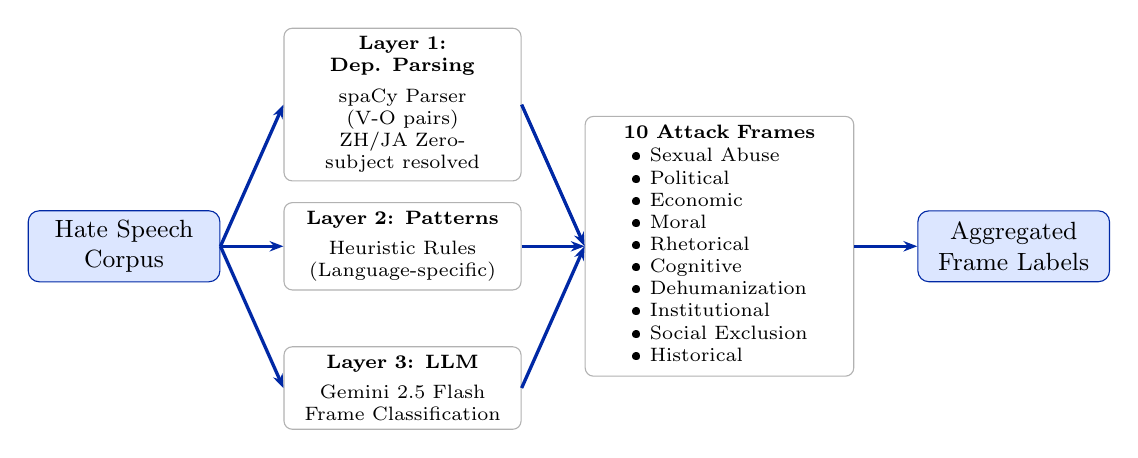
\begin{tikzpicture}[node distance=0.5cm and 0.8cm]
      \node[mbox=2.2cm] (inp) {Hate Speech\\Corpus};
    
      % --- 三层提取结构 (增加 yshift 以防重叠) ---
      \node[sbox=2.8cm, right=0.8cm of inp, yshift=1.8cm] (l1)
        {\textbf{Layer 1: Dep. Parsing}\\[3pt]
         {\scriptsize spaCy Parser (V-O pairs)\\
         ZH/JA Zero-subject resolved}};
    
      \node[sbox=2.8cm, right=0.8cm of inp] (l2)
        {\textbf{Layer 2: Patterns}\\[3pt]
         {\scriptsize Heuristic Rules\\
         (Language-specific)}};
    
      \node[sbox=2.8cm, right=0.8cm of inp, yshift=-1.8cm] (l3)
        {\textbf{Layer 3: LLM}\\[3pt]
         {\scriptsize Gemini 2.5 Flash\\
         Frame Classification}};
    
      \draw[arr] (inp.east) -- (l1.west);
      \draw[arr] (inp.east) -- (l2.west);
      \draw[arr] (inp.east) -- (l3.west);
    
      % --- 10类分类体系 (精简文字) ---
      \node[sbox=3.2cm, right=0.8cm of l2] (tax)
        {\textbf{10 Attack Frames}\\[2pt]
         \begin{tabular}{ll}
           • Sexual Abuse \\ • Political \\
           • Economic \\ • Moral \\
           • Rhetorical \\ • Cognitive \\
           • Dehumanization \\ • Institutional \\
           • Social Exclusion \\ • Historical
         \end{tabular}};
    
      \draw[arr] (l1.east) -- (tax.west);
      \draw[arr] (l2.east) -- (tax.west);
      \draw[arr] (l3.east) -- (tax.west);
    
      % --- 输出 ---
      \node[mbox=2.2cm, right=0.8cm of tax] (out)
        {Aggregated\\Frame Labels};
    
      \draw[arr] (tax)--(out);
    \end{tikzpicture}
  \end{center}
\end{frame}

% ── SLIDE 13 · RQ2 by language ───────────────────────────────
\begin{frame}{RQ2 --- Results: Frame Distribution by Language}
  \begin{columns}[T]
    \column{0.58\textwidth}
      
\includegraphics[width=\linewidth]{images/RQ2/rq2_lang_tactic.png}
      {\tiny 10-frame distribution by language community (predicate counts).}
    \column{0.38\textwidth}
      \vspace{4pt}
      \begin{block}{\small EN --- Rhetoric \& moral condemnation}
        {\footnotesize
        Rhetorical Attack (46\%),\\
        Moral Accusation (22\%),\\
        Sexual Abuse (14\%)}
      \end{block}
      \vspace{4pt}
      \begin{block}{\small JA --- Political \& economic frames}
        {\footnotesize
        Political Interference (20\%),\\
        Rhetorical Attack (18\%),\\
        Economic Exploitation (14\%)\\
        \textit{Driven by Abe/Unification Church}}
      \end{block}
      \vspace{4pt}
      \begin{block}{\small ZH --- Sexual abuse salient}
        {\footnotesize
        Sexual Abuse Frame (26\%),\\
        Rhetorical Attack (25\%),\\
        Moral Accusation (14\%)}
      \end{block}
  \end{columns}
\end{frame}

% ── SLIDE 14 · RQ2 target--tactic (key finding) ──────────────
\begin{frame}{RQ2 --- Key Finding: Frame = Target Type, Not Language}
  \begin{columns}[T]
    \column{0.55\textwidth}
      
\includegraphics[width=\linewidth]{images/RQ2/rq2_target_tactic.png}
      {\tiny Attack-frame distribution by target entity (all languages pooled).}
    \column{0.42\textwidth}
      \vspace{6pt}
      \begin{alertblock}{\faExclamationTriangle\ Structural regularity \#1}
        Frame choice is governed by the\\
        \textbf{target's social category},\\
        not by language community.
      \end{alertblock}
      \vspace{6pt}
      \begin{block}{Cross-lingual genre conventions}
        \small
        \begin{tabular}{@{}ll@{}}
          \toprule
          \textbf{Target type} & \textbf{Dominant frame} \\
          \midrule
          Clergy roles & Sexual Abuse \\
          Church institution & Institutional Rot \\
          Political institution & Political Interf. \\
          Collective identity & Rhetorical Attack \\
          Collective identity & Moral Accusation \\
          \bottomrule
        \end{tabular}
      \end{block}
      \vspace{4pt}
      {\footnotesize Holds independently in EN, ZH \& JA.}
  \end{columns}
\end{frame}

% ============================================================
\section{RQ3 --- Why? Method \& Results}
% ============================================================

% ── SLIDE 15 · RQ3 Method ────────────────────────────────────
\begin{frame}{RQ3 --- Method: Moral Axis Projection}
  \begin{center}
    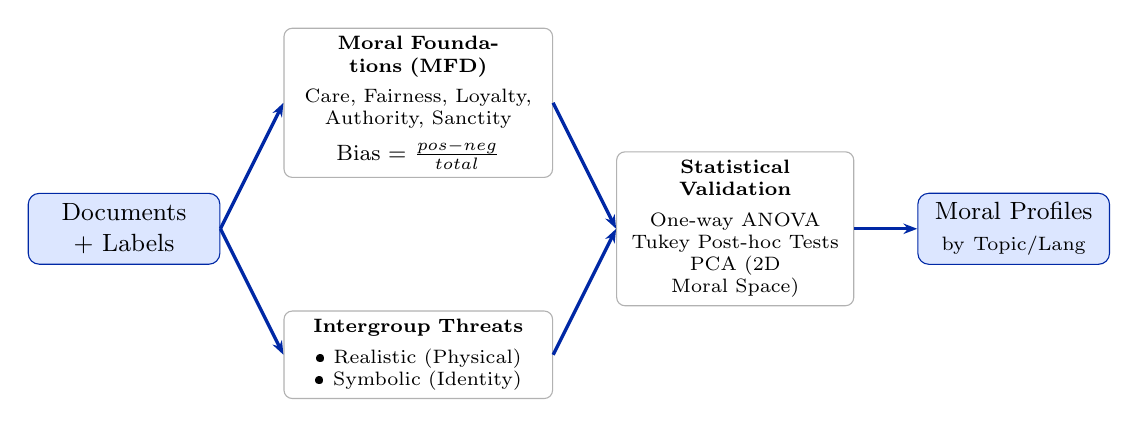
\begin{tikzpicture}[node distance=0.5cm and 0.8cm]
      \node[mbox=2.2cm] (inp) {Documents\\+ Labels};
    
      % --- 上分支：MFD (增加 yshift，精简字典内容) ---
      \node[sbox=3.2cm, right=0.8cm of inp, yshift=1.6cm] (mft)
        {\textbf{Moral Foundations (MFD)}\\[3pt]
         {\scriptsize Care, Fairness, Loyalty,\\Authority, Sanctity}\\[3pt]
         {\footnotesize Bias = $\frac{pos - neg}{total}$}};
    
      % --- 下分支：Threats (增加 yshift) ---
      \node[sbox=3.2cm, right=0.8cm of inp, yshift=-1.6cm] (thr)
        {\textbf{Intergroup Threats}\\[3pt]
         {\scriptsize \textbullet\ Realistic (Physical)\\
         \textbullet\ Symbolic (Identity)}};
    
      \draw[arr] (inp.east) -- (mft.west);
      \draw[arr] (inp.east) -- (thr.west);
    
      % --- 统计验证 (精简数据指标) ---
      \node[sbox=2.8cm, right=0.8cm of mft, yshift=-1.6cm] (stat)
        {\textbf{Statistical Validation}\\[3pt]
         {\scriptsize One-way ANOVA\\
         Tukey Post-hoc Tests\\
         PCA (2D Moral Space)}};
    
      \draw[arr] (mft.east) -- (stat.west);
      \draw[arr] (thr.east) -- (stat.west);
    
      % --- 输出 (更紧凑) ---
      \node[mbox=2.2cm, right=0.8cm of stat] (out)
        {Moral Profiles\\{\scriptsize by Topic/Lang}};
    
      \draw[arr] (stat)--(out);
    \end{tikzpicture}
  \end{center}
  \vspace{6pt}
  \begin{block}{}
    \small\centering
    \textbf{Interpretation:} a \emph{negative} score means the discourse invokes the\\
    attack-oriented pole of that foundation (e.g., \emph{Harm} rather than \emph{Care}).
  \end{block}
\end{frame}

% ── SLIDE 16 · RQ3 language profiles ─────────────────────────
\begin{frame}{RQ3 --- Results: Different Moral Vocabularies}

  \begin{columns}[T]
    \column{0.58\textwidth}
      \vspace{2pt}
        \begin{tikzpicture}
          \begin{axis}[
            width=8.5cm, height=6.5cm,
            ylabel={Mean Bias Score},
            xlabel={Moral Dimensions},
            % 设置维度刻度
            symbolic x coords={Harm, Fairness, Loyalty, Authority, Sanctity, Realistic Threat, Symbolic Threat},
            xtick=data,
            % 标签旋转 30 度避免重叠，字体调小
            x tick label style={rotate=30, anchor=north east, font=\tiny},
            y tick label style={font=\small},
            % 坐标轴范围与参考线
            ymin=-0.15, ymax=0.25,
            ytick={-0.1, -0.05, 0, 0.05, 0.1, 0.15, 0.2},
            extra y ticks={0}, % 突出 0 线
            extra y tick style={grid=major, grid style={thick, black!60}},
            ymajorgrids=true, grid style={dashed, gray!30},
            % 图例设置
            legend style={at={(0.5,-0.25)}, anchor=north, legend columns=3, font=\scriptsize},
            title={\small Moral & Threat Profiles by Language},
          ]
            
            % ── EN (使用原有颜色 enzh)
            \addplot[color=enzh, mark=*, thick] coordinates {
              (Harm,-0.074) (Fairness,-0.063) (Loyalty,-0.050) 
              (Authority,-0.081) (Sanctity,-0.065) 
              (Realistic Threat,0.018) (Symbolic Threat,-0.022)
            };
        
            % ── ZH (使用原有颜色 zhcol)
            \addplot[color=zhcol!120, mark=square*, thick] coordinates {
              (Harm,0.177) (Fairness,0.182) (Loyalty,0.108) 
              (Authority,0.117) (Sanctity,0.168) 
              (Realistic Threat,-0.012) (Symbolic Threat,-0.047)
            };
        
            % ── JA (使用原有颜色 jacol)
            \addplot[color=jacol!120, mark=triangle*, thick] coordinates {
              (Harm,0.069) (Fairness,0.085) (Loyalty,0.024) 
              (Authority,0.034) (Sanctity,0.077) 
              (Realistic Threat,-0.018) (Symbolic Threat,-0.045)
            };
        
            \legend{EN (English), ZH (Chinese), JA (Japanese)}
          \end{axis}
        \end{tikzpicture}

    \column{0.38\textwidth}
      \vspace{4pt}
      \begin{alertblock}{\faExclamationTriangle\ Structural regularity \#2}
        \textbf{English:} negative across all\\
        5 classical MFT axes\\
        $\Rightarrow$ \emph{broad ethical condemnation}\\[8pt]
        \textbf{ZH \& JA:} positive on MFT,\\
        negative only on\\
        Symbolic + Realistic \emph{Threat}\\
        $\Rightarrow$ \emph{identity-threat framing}
      \end{alertblock}
      \begin{block}{Statistical validation}
        \footnotesize
        All 7 axes: ANOVA\\
        $p < 4.9 \times 10^{-324}$\\
        $\eta^2 = 0.24$--$0.95$\\[4pt]
        EN is the \textbf{only} language\\
        where Realistic Threat\\
        is \emph{positive} ($+0.018$).
      \end{block}
  \end{columns}
\end{frame}

% ── SLIDE 17 · RQ3 moral architecture ────────────────────────
\begin{frame}{RQ3 --- Results: Two Moral Universes}
  \begin{columns}[T]
    \column{0.58\textwidth}
      \vspace{4pt}
      % 2D moral space: X = MFT condemnation, Y = threat framing
      % EN:  MFT avg = -0.067,  Threat avg = -0.002
      % ZH:  MFT avg = +0.150,  Threat avg = -0.030
      % JA:  MFT avg = +0.058,  Threat avg = -0.032
      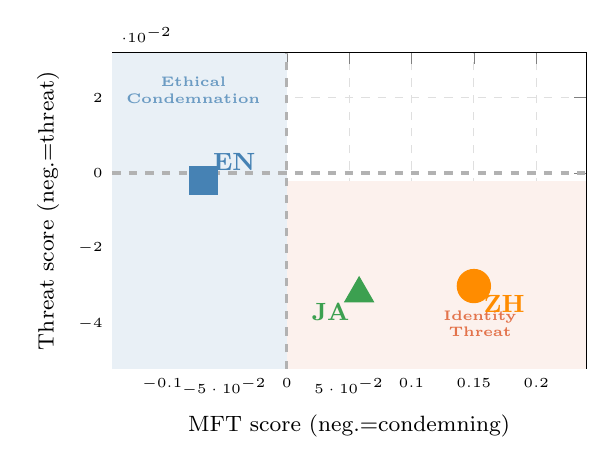
\begin{tikzpicture}
        \begin{axis}[
          width=7.6cm, height=5.6cm,
          xlabel={\footnotesize MFT score (neg.$=$condemning)},
          ylabel={\footnotesize Threat score (neg.$=$threat)},
          xmin=-0.14, xmax=0.24,
          ymin=-0.052, ymax=0.032,
          xtick={-0.10,-0.05,0.00,0.05,0.10,0.15,0.20},
          ytick={-0.04,-0.02,0.00,0.02},
          x tick label style={font=\tiny},
          y tick label style={font=\tiny},
          xlabel style={font=\small},
          ylabel style={font=\small},
          grid=both, grid style={dashed,gray!25},
          clip=false,
        ]
          % Quadrant shading
          \fill[enzh!12] (-0.14,-0.052) rectangle (0.00, 0.032);
          \fill[accent!8]  (0.00,-0.052) rectangle (0.24,-0.002);
          % Reference lines
          \draw[very thick,gray!60,dashed] (axis cs:0,-0.052)--(axis cs:0,0.032);
          \draw[very thick,gray!60,dashed] (axis cs:-0.14,0)--(axis cs:0.24,0);
          % Quadrant labels
          \node[font=\tiny\bfseries,color=enzh!80,align=center]
            at (axis cs:-0.075, 0.022) {Ethical\\Condemnation};
          \node[font=\tiny\bfseries,color=accent!80,align=center]
            at (axis cs:0.155, -0.040) {Identity\\Threat};
          % EN
          \addplot[only marks,mark=square*,mark size=5pt,color=enzh]
            coordinates {(-0.067,-0.002)};
          \node[font=\small\bfseries,color=enzh,anchor=south west]
            at (axis cs:-0.067,-0.002) {EN};
          % ZH
          \addplot[only marks,mark=*,mark size=6pt,color=zhcol]
            coordinates {(0.150,-0.030)};
          \node[font=\small\bfseries,color=zhcol,anchor=north west]
            at (axis cs:0.150,-0.030) {ZH};
          % JA
          \addplot[only marks,mark=triangle*,mark size=6pt,color=jacol]
            coordinates {(0.058,-0.032)};
          \node[font=\small\bfseries,color=jacol,anchor=north east]
            at (axis cs:0.058,-0.032) {JA};
        \end{axis}
      \end{tikzpicture}\\
      {\tiny X = mean of 5 MFT axes; Y = mean of 2 threat axes.
             All differences significant ($p < 10^{-200}$).}
    \column{0.38\textwidth}
      \vspace{6pt}
      \begin{block}{English speakers say:}
        \small ``Christianity is \emph{morally wrong}''\\[4pt]
        Wide ethical condemnation\\
        using \emph{shared} normative standards\\
        (insider critique)
      \end{block}
      \vspace{6pt}
      \begin{alertblock}{East Asian speakers say:}
        \small ``Christianity is \emph{dangerous to us}''\\[4pt]
        Cultural invasion /\\
        social threat framing\\
        (outsider critique, group safety)
      \end{alertblock}
      \vspace{6pt}
      \textbf{\small Same target.\\Fundamentally different moral logic.}
  \end{columns}
\end{frame}

% ============================================================
\section{Discussion}
% ============================================================

% ── SLIDE 18 · Discussion -- two regularities ─────────────────
\begin{frame}{Discussion: Two Structural Regularities}
  \begin{columns}[T]
    % ── LEFT: Genre convention map (TikZ) ──────────────────────
    \column{0.54\textwidth}
      \begin{block}{\#1 --- Attack Frames as Genre Conventions}
        \footnotesize
        Frame choice is governed by \textbf{target type}, not language.\\
        Same conventions hold in EN, ZH \& JA.
      \end{block}
      \vspace{4pt}
      \begin{center}
      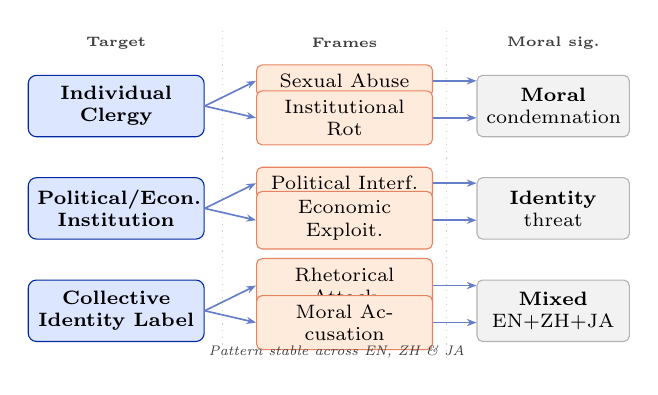
\begin{tikzpicture}[
        tgt/.style={rectangle,rounded corners=3pt,draw=uzh,fill=uzhlight,
                    text width=2.0cm,align=center,minimum height=0.78cm,
                    font=\scriptsize\bfseries},
        frm/.style={rectangle,rounded corners=2pt,draw=accent!70,fill=accentlt,
                    text width=2.0cm,align=center,minimum height=0.36cm,
                    font=\scriptsize},
        mor/.style={rectangle,rounded corners=2pt,draw=gray!60,fill=gray!10,
                    text width=1.7cm,align=center,minimum height=0.78cm,
                    font=\scriptsize},
        ca/.style={-{Stealth[length=3.5pt]},semithick,color=uzh!60},
      ]
        % ── Column headers
        \node[font=\tiny\bfseries,color=darkgray] at (0,    3.0) {Target};
        \node[font=\tiny\bfseries,color=darkgray] at (2.9,  3.0) {Frames};
        \node[font=\tiny\bfseries,color=darkgray] at (5.55, 3.0) {Moral sig.};
        \draw[gray!40,dotted] (1.35,3.15)--(1.35,-1.0);
        \draw[gray!40,dotted] (4.2, 3.15)--(4.2, -1.0);

        % ── Row 1 : Individual Clergy
        \node[tgt] (t1) at (0,    2.2) {Individual\\Clergy};
        \node[frm] (f1a) at (2.9, 2.52) {Sexual Abuse};
        \node[frm] (f1b) at (2.9, 2.05) {Institutional Rot};
        \node[mor] (m1)  at (5.55,2.2)  {\textbf{Moral}\\condemnation};

        % ── Row 2 : Institution
        \node[tgt] (t2) at (0,    0.9) {Political/Econ.\\Institution};
        \node[frm] (f2a) at (2.9, 1.22) {Political Interf.};
        \node[frm] (f2b) at (2.9, 0.75) {Economic Exploit.};
        \node[mor] (m2)  at (5.55,0.9)  {\textbf{Identity}\\threat};

        % ── Row 3 : Collective identity
        \node[tgt] (t3) at (0,   -0.4) {Collective\\Identity Label};
        \node[frm] (f3a) at (2.9,-0.08) {Rhetorical Attack};
        \node[frm] (f3b) at (2.9,-0.55) {Moral Accusation};
        \node[mor] (m3)  at (5.55,-0.4) {\textbf{Mixed}\\EN+ZH+JA};

        % ── Arrows
        \draw[ca] (t1.east)--(f1a.west); \draw[ca] (t1.east)--(f1b.west);
        \draw[ca] (t2.east)--(f2a.west); \draw[ca] (t2.east)--(f2b.west);
        \draw[ca] (t3.east)--(f3a.west); \draw[ca] (t3.east)--(f3b.west);
        \draw[ca] (f1a.east)--(m1.west|-f1a.east);
        \draw[ca] (f1b.east)--(m1.west|-f1b.east);
        \draw[ca] (f2a.east)--(m2.west|-f2a.east);
        \draw[ca] (f2b.east)--(m2.west|-f2b.east);
        \draw[ca] (f3a.east)--(m3.west|-f3a.east);
        \draw[ca] (f3b.east)--(m3.west|-f3b.east);

        % ── Footer
        \node[font=\tiny\itshape,text=darkgray,align=center]
          at (2.8,-0.92) {Pattern stable across EN, ZH \& JA};
      \end{tikzpicture}
      \end{center}

    % ── RIGHT: Moral architecture summary ──────────────────────
    \column{0.43\textwidth}
      \begin{block}{\#2 --- Two Moral Architectures}
        \small
        EN: \emph{moral transgressor} model\\
        --- Christianity judged by\\
        universal ethical standards.\\[5pt]
        ZH/JA: \emph{outgroup threat} model\\
        --- Christianity is a\\
        cultural/social danger.\\[5pt]
        Binary classifiers collapse this\\
        difference; structured analysis\\
        makes it visible.
      \end{block}
      \vspace{6pt}
      \begin{alertblock}{Broader lesson}
        \small
        Binary detection cannot surface\\
        these structural patterns.\\
        \textbf{The who--how--why pipeline can.}
      \end{alertblock}
  \end{columns}
\end{frame}

% ── SLIDE 19 · Methodological reflections ────────────────────
\begin{frame}{Discussion: Methodological Reflections}
  \begin{columns}[T]
    \column{0.48\textwidth}
      \begin{block}{What worked}
        \small
        \begin{itemize}
          \item \textbf{Double BT} resolves distribution shift --- reusable solution for low-resource hate speech
          \item \textbf{Cross-lingual centroid alignment} in BERTopic creates genuinely mixed topics without translation
          \item \textbf{Corpus-induction} lets culturally specific topics emerge naturally (JP Unification Church)
        \end{itemize}
      \end{block}
    \column{0.48\textwidth}
      \begin{alertblock}{What to watch for}
        \small
        \begin{itemize}
          \item \textbf{LLM data collapse}: after 20--30 iterations, ZH/JA generation becomes 90--100\% redundant
          \item \textbf{Platform bias}: Tieba (ZH) and 5ch (JA) are not representative of all online speech
          \item \textbf{Annotation noise}: implicit hate labels have moderate inter-annotator agreement
        \end{itemize}
      \end{alertblock}
  \end{columns}
\end{frame}

% ============================================================
\section{Contributions, Limitations \& Outlook}
% ============================================================

% ── SLIDE 20 · Contributions ─────────────────────────────────
\begin{frame}{Contributions}
  \begin{columns}[T]
    \column{0.31\textwidth}
      \begin{block}{Resource}
        \small
        First trilingual corpus of anti-Christian hate speech (EN/ZH/JA, 63,265 texts)\\[4pt]
        Structured annotation:\\
        target $\times$ frame $\times$ moral axis\\[4pt]
        \textbf{Open-source on GitHub}
      \end{block}
    \column{0.31\textwidth}
      \begin{block}{Empirical}
        \small
        First systematic cross-lingual analysis revealing:\\[4pt]
        (1) Attack frame $=$ genre convention\\[4pt]
        (2) EN vs.\ EA communities inhabit different moral universes
      \end{block}
    \column{0.31\textwidth}
      \begin{block}{Methodological}
        \small
        Reusable \textbf{who--how--why} pipeline:\\[4pt]
        multilingual embeddings,\\
        topic modelling,\\
        frame classification,\\
        moral-axis projection\\[4pt]
        All code open-source
      \end{block}
  \end{columns}
\end{frame}

% ── SLIDE 21 · Limitations & Future Work ─────────────────────
\begin{frame}{Limitations \& Future Work}
  \begin{columns}[T]
    \column{0.48\textwidth}
      \begin{alertblock}{Current limitations}
        \begin{itemize}\small
          \item \textbf{Platform coverage}: Tieba \& 5ch may not generalise to WeChat, Twitter/X, LINE
          \item \textbf{Temporal snapshot}: discourse evolves --- longitudinal re-running needed
          \item \textbf{ZH/JA corpus size}: still small despite augmentation
          \item \textbf{Annotation noise}: implicit hate labels are harder to label consistently
        \end{itemize}
      \end{alertblock}
    \column{0.48\textwidth}
      \begin{block}{Promising directions}
        \begin{itemize}\small
          \item Apply pipeline to \textbf{other religious minorities} (Islamophobia, antisemitism) --- same framework, different case
          \item \textbf{More languages} (Korean, Vietnamese): does the moral-architecture split generalise?
          \item \textbf{Larger LLMs with RAG} for stable low-resource augmentation
          \item \textbf{Longitudinal analysis}: does moral framing shift after major events? (post-2022 Abe assassination)
        \end{itemize}
      \end{block}
  \end{columns}
\end{frame}

% ── SLIDE 22 · Summary ───────────────────────────────────────
\begin{frame}{Summary: The Story in Three Acts}
  \begin{columns}[T]
    \column{0.32\textwidth}
      \begin{block}{Act 1 --- Data}
        \small
        Built a trilingual corpus\\
        from near-zero.\\[4pt]
        Back-translation solved\\
        the low-resource problem\\
        better than LLM generation.
      \end{block}
    \column{0.32\textwidth}
      \begin{block}{Act 2 --- Structure}
        \small
        Frame selection follows\\
        the target, not the language.\\[4pt]
        Cross-cultural genre\\
        conventions exist in\\
        hate speech.
      \end{block}
    \column{0.32\textwidth}
      \begin{alertblock}{Act 3 --- Morality}
        \small
        \textbf{English} condemns.\\
        \textbf{East Asian} fears.\\[4pt]
        Same target, fundamentally\\
        different moral logic ---\\
        invisible to binary detectors.
      \end{alertblock}
  \end{columns}
  \vspace{10pt}
  \begin{center}
    \small\texttt{github.com/notsofun/Master\_Thesis}\\[4pt]
    {\footnotesize\color{darkgray} Open-source corpus, annotations, and pipeline code}
  \end{center}
\end{frame}

% ── SLIDE 23 · Q\&A ───────────────────────────────────────────
\begin{frame}[plain]
  \begin{center}
    \vspace{1.5cm}
    {\Huge\color{uzh} Thank you.}\\[20pt]
    {\Large Questions?}\\[24pt]
    \small
    Zhidian Huang\\
    \texttt{huangzhidian15@gmail.com}\\[8pt]
    \texttt{github.com/notsofun/Master\_Thesis}
  \end{center}
\end{frame}

% ── References ───────────────────────────────────────────────
% \begin{frame}[allowframebreaks]{Selected References}
%     \subfilebibliography
% \end{frame}

\end{document}
